% Generated by Sphinx.
\def\sphinxdocclass{report}
\documentclass[letterpaper,10pt,brazil]{sphinxmanual}
\usepackage[utf8]{inputenc}
\DeclareUnicodeCharacter{00A0}{\nobreakspace}
\usepackage[T1]{fontenc}
\usepackage{babel}
\usepackage{times}
\usepackage[Sonny]{fncychap}
\usepackage{longtable}
\usepackage{sphinx}
\usepackage{multirow}


\title{PABX IP Documentation}
\date{20/03/2012}
\release{0.1}
\author{Fabio Hiroki}
\newcommand{\sphinxlogo}{}
\renewcommand{\releasename}{Versão}
\makeindex

\makeatletter
\def\PYG@reset{\let\PYG@it=\relax \let\PYG@bf=\relax%
    \let\PYG@ul=\relax \let\PYG@tc=\relax%
    \let\PYG@bc=\relax \let\PYG@ff=\relax}
\def\PYG@tok#1{\csname PYG@tok@#1\endcsname}
\def\PYG@toks#1+{\ifx\relax#1\empty\else%
    \PYG@tok{#1}\expandafter\PYG@toks\fi}
\def\PYG@do#1{\PYG@bc{\PYG@tc{\PYG@ul{%
    \PYG@it{\PYG@bf{\PYG@ff{#1}}}}}}}
\def\PYG#1#2{\PYG@reset\PYG@toks#1+\relax+\PYG@do{#2}}

\def\PYG@tok@gd{\def\PYG@tc##1{\textcolor[rgb]{0.63,0.00,0.00}{##1}}}
\def\PYG@tok@gu{\let\PYG@bf=\textbf\def\PYG@tc##1{\textcolor[rgb]{0.50,0.00,0.50}{##1}}}
\def\PYG@tok@gt{\def\PYG@tc##1{\textcolor[rgb]{0.00,0.25,0.82}{##1}}}
\def\PYG@tok@gs{\let\PYG@bf=\textbf}
\def\PYG@tok@gr{\def\PYG@tc##1{\textcolor[rgb]{1.00,0.00,0.00}{##1}}}
\def\PYG@tok@cm{\let\PYG@it=\textit\def\PYG@tc##1{\textcolor[rgb]{0.25,0.50,0.56}{##1}}}
\def\PYG@tok@vg{\def\PYG@tc##1{\textcolor[rgb]{0.73,0.38,0.84}{##1}}}
\def\PYG@tok@m{\def\PYG@tc##1{\textcolor[rgb]{0.13,0.50,0.31}{##1}}}
\def\PYG@tok@mh{\def\PYG@tc##1{\textcolor[rgb]{0.13,0.50,0.31}{##1}}}
\def\PYG@tok@cs{\def\PYG@tc##1{\textcolor[rgb]{0.25,0.50,0.56}{##1}}\def\PYG@bc##1{\colorbox[rgb]{1.00,0.94,0.94}{##1}}}
\def\PYG@tok@ge{\let\PYG@it=\textit}
\def\PYG@tok@vc{\def\PYG@tc##1{\textcolor[rgb]{0.73,0.38,0.84}{##1}}}
\def\PYG@tok@il{\def\PYG@tc##1{\textcolor[rgb]{0.13,0.50,0.31}{##1}}}
\def\PYG@tok@go{\def\PYG@tc##1{\textcolor[rgb]{0.19,0.19,0.19}{##1}}}
\def\PYG@tok@cp{\def\PYG@tc##1{\textcolor[rgb]{0.00,0.44,0.13}{##1}}}
\def\PYG@tok@gi{\def\PYG@tc##1{\textcolor[rgb]{0.00,0.63,0.00}{##1}}}
\def\PYG@tok@gh{\let\PYG@bf=\textbf\def\PYG@tc##1{\textcolor[rgb]{0.00,0.00,0.50}{##1}}}
\def\PYG@tok@ni{\let\PYG@bf=\textbf\def\PYG@tc##1{\textcolor[rgb]{0.84,0.33,0.22}{##1}}}
\def\PYG@tok@nl{\let\PYG@bf=\textbf\def\PYG@tc##1{\textcolor[rgb]{0.00,0.13,0.44}{##1}}}
\def\PYG@tok@nn{\let\PYG@bf=\textbf\def\PYG@tc##1{\textcolor[rgb]{0.05,0.52,0.71}{##1}}}
\def\PYG@tok@no{\def\PYG@tc##1{\textcolor[rgb]{0.38,0.68,0.84}{##1}}}
\def\PYG@tok@na{\def\PYG@tc##1{\textcolor[rgb]{0.25,0.44,0.63}{##1}}}
\def\PYG@tok@nb{\def\PYG@tc##1{\textcolor[rgb]{0.00,0.44,0.13}{##1}}}
\def\PYG@tok@nc{\let\PYG@bf=\textbf\def\PYG@tc##1{\textcolor[rgb]{0.05,0.52,0.71}{##1}}}
\def\PYG@tok@nd{\let\PYG@bf=\textbf\def\PYG@tc##1{\textcolor[rgb]{0.33,0.33,0.33}{##1}}}
\def\PYG@tok@ne{\def\PYG@tc##1{\textcolor[rgb]{0.00,0.44,0.13}{##1}}}
\def\PYG@tok@nf{\def\PYG@tc##1{\textcolor[rgb]{0.02,0.16,0.49}{##1}}}
\def\PYG@tok@si{\let\PYG@it=\textit\def\PYG@tc##1{\textcolor[rgb]{0.44,0.63,0.82}{##1}}}
\def\PYG@tok@s2{\def\PYG@tc##1{\textcolor[rgb]{0.25,0.44,0.63}{##1}}}
\def\PYG@tok@vi{\def\PYG@tc##1{\textcolor[rgb]{0.73,0.38,0.84}{##1}}}
\def\PYG@tok@nt{\let\PYG@bf=\textbf\def\PYG@tc##1{\textcolor[rgb]{0.02,0.16,0.45}{##1}}}
\def\PYG@tok@nv{\def\PYG@tc##1{\textcolor[rgb]{0.73,0.38,0.84}{##1}}}
\def\PYG@tok@s1{\def\PYG@tc##1{\textcolor[rgb]{0.25,0.44,0.63}{##1}}}
\def\PYG@tok@gp{\let\PYG@bf=\textbf\def\PYG@tc##1{\textcolor[rgb]{0.78,0.36,0.04}{##1}}}
\def\PYG@tok@sh{\def\PYG@tc##1{\textcolor[rgb]{0.25,0.44,0.63}{##1}}}
\def\PYG@tok@ow{\let\PYG@bf=\textbf\def\PYG@tc##1{\textcolor[rgb]{0.00,0.44,0.13}{##1}}}
\def\PYG@tok@sx{\def\PYG@tc##1{\textcolor[rgb]{0.78,0.36,0.04}{##1}}}
\def\PYG@tok@bp{\def\PYG@tc##1{\textcolor[rgb]{0.00,0.44,0.13}{##1}}}
\def\PYG@tok@c1{\let\PYG@it=\textit\def\PYG@tc##1{\textcolor[rgb]{0.25,0.50,0.56}{##1}}}
\def\PYG@tok@kc{\let\PYG@bf=\textbf\def\PYG@tc##1{\textcolor[rgb]{0.00,0.44,0.13}{##1}}}
\def\PYG@tok@c{\let\PYG@it=\textit\def\PYG@tc##1{\textcolor[rgb]{0.25,0.50,0.56}{##1}}}
\def\PYG@tok@mf{\def\PYG@tc##1{\textcolor[rgb]{0.13,0.50,0.31}{##1}}}
\def\PYG@tok@err{\def\PYG@bc##1{\fcolorbox[rgb]{1.00,0.00,0.00}{1,1,1}{##1}}}
\def\PYG@tok@kd{\let\PYG@bf=\textbf\def\PYG@tc##1{\textcolor[rgb]{0.00,0.44,0.13}{##1}}}
\def\PYG@tok@ss{\def\PYG@tc##1{\textcolor[rgb]{0.32,0.47,0.09}{##1}}}
\def\PYG@tok@sr{\def\PYG@tc##1{\textcolor[rgb]{0.14,0.33,0.53}{##1}}}
\def\PYG@tok@mo{\def\PYG@tc##1{\textcolor[rgb]{0.13,0.50,0.31}{##1}}}
\def\PYG@tok@mi{\def\PYG@tc##1{\textcolor[rgb]{0.13,0.50,0.31}{##1}}}
\def\PYG@tok@kn{\let\PYG@bf=\textbf\def\PYG@tc##1{\textcolor[rgb]{0.00,0.44,0.13}{##1}}}
\def\PYG@tok@o{\def\PYG@tc##1{\textcolor[rgb]{0.40,0.40,0.40}{##1}}}
\def\PYG@tok@kr{\let\PYG@bf=\textbf\def\PYG@tc##1{\textcolor[rgb]{0.00,0.44,0.13}{##1}}}
\def\PYG@tok@s{\def\PYG@tc##1{\textcolor[rgb]{0.25,0.44,0.63}{##1}}}
\def\PYG@tok@kp{\def\PYG@tc##1{\textcolor[rgb]{0.00,0.44,0.13}{##1}}}
\def\PYG@tok@w{\def\PYG@tc##1{\textcolor[rgb]{0.73,0.73,0.73}{##1}}}
\def\PYG@tok@kt{\def\PYG@tc##1{\textcolor[rgb]{0.56,0.13,0.00}{##1}}}
\def\PYG@tok@sc{\def\PYG@tc##1{\textcolor[rgb]{0.25,0.44,0.63}{##1}}}
\def\PYG@tok@sb{\def\PYG@tc##1{\textcolor[rgb]{0.25,0.44,0.63}{##1}}}
\def\PYG@tok@k{\let\PYG@bf=\textbf\def\PYG@tc##1{\textcolor[rgb]{0.00,0.44,0.13}{##1}}}
\def\PYG@tok@se{\let\PYG@bf=\textbf\def\PYG@tc##1{\textcolor[rgb]{0.25,0.44,0.63}{##1}}}
\def\PYG@tok@sd{\let\PYG@it=\textit\def\PYG@tc##1{\textcolor[rgb]{0.25,0.44,0.63}{##1}}}

\def\PYGZbs{\char`\\}
\def\PYGZus{\char`\_}
\def\PYGZob{\char`\{}
\def\PYGZcb{\char`\}}
\def\PYGZca{\char`\^}
\def\PYGZsh{\char`\#}
\def\PYGZpc{\char`\%}
\def\PYGZdl{\char`\$}
\def\PYGZti{\char`\~}
% for compatibility with earlier versions
\def\PYGZat{@}
\def\PYGZlb{[}
\def\PYGZrb{]}
\makeatother

\begin{document}

\maketitle
\tableofcontents
\phantomsection\label{index::doc}



\chapter{Introdução}
\label{index:bem-vindo-a-documentacao-do-projeto-pabx-ip}\label{index:introducao}
Esta documentação tem o objetivo de servir de base para auxiliar o entendimento do código-fonte do projeto PABX-IP, facilitando as futuras extensões de funcionalidades a serem desenvolvidas.


\chapter{Recomendações}
\label{index:recomendacoes}
Antes de mais nada, o desenvolvedor deve estar a par da documentação das funcionalidades do PABX que é outro documento separado desse. Alguns diagramas de fluxo e esboço de telas também foram feitos também, mas é bem provável que estes estejam desatualizados agora.

Para entendimento do código e dessa documentação é importante que o leitor tenha um conhecimento geral de programação orientada a objetos, banco de dados e desenvolvimento web. É indispensável um conhecimento prévio no framework Django.


\chapter{Conteúdo}
\label{index:conteudo}

\section{Para começar}
\label{inicio::doc}\label{inicio:para-comecar}
Nessa seção será mostrado as ferramentas que são pré-requisitos para desenvolvimento do projeto. Também mostraremos como instalá-las e configurá-las corretamente, para que o desenvolvedor já consiga ao menos rodar o PABX-IP em sua máquina local.


\subsection{Ambiente de Desenvolvimento}
\label{inicio:ambiente-de-desenvolvimento}\begin{itemize}
\item {} 
Sistema Operacional (recomendável): Ubuntu

\item {} 
Python 2.7 (a versão 3 é incompatível com outras bibliotecas)

\item {} 
Framework Django + Pinax

\item {} 
Banco de dados SQLite

\item {} 
Conexão com a internet

\end{itemize}


\subsection{Instalação do ambiente de desenvolvimento}
\label{inicio:instalacao-do-ambiente-de-desenvolvimento}
Esse tutorial foi feito no Ubuntu 10.04, usando o repositório git onde o código estava sendo versionado na época em que essa documentação foi feita. Caso o desenvolvedor já possua o código fonte, pule a parte 1.


\subsubsection{Instalação do git e clone do repositório:}
\label{inicio:instalacao-do-git-e-clone-do-repositorio}
\begin{Verbatim}[commandchars=\\\{\}]
\$ sudo apt-get install git-core

\$ git clone https://github.com/fabiothiroki/pabx\_ip.git
\end{Verbatim}


\subsubsection{Instalação e ativação do virtualenv:}
\label{inicio:instalacao-e-ativacao-do-virtualenv}
O virtualenv é uma ferramenta de criação de ambientes python isolados. Isso visa facilitar o deploy da aplicação.

Toda vez que o desenvolvedor quiser rodar o servidor local de desenvolvimento do django é necessário ativar esse ambiente, pois é nele que estarão instalados o Pinax e as bibliotecas python auxiliares.

Antes de mais nada é interessante que todas as bibliotecas do OS sejam atualizadas

\begin{Verbatim}[commandchars=\\\{\}]
\$ sudo apt-get update
\$ sudo apt-get dist-update
\end{Verbatim}

Agora então vamos a instalação do virtualenv:

\begin{Verbatim}[commandchars=\\\{\}]
\$ sudo apt-get install python-pip

\$ sudo pip install virtualenv

\$ virtualenv pabx-env

\$ source pabx-env/bin/activate
\end{Verbatim}


\subsubsection{Instalação do Pinax e outros apps:}
\label{inicio:instalacao-do-pinax-e-outros-apps}
Pinax é uma plataforma baseada no Django que contém diversos apps pré-instalados.

Para mais informações consulte: \href{http://pinaxproject.com/}{http://pinaxproject.com/}

\begin{Verbatim}[commandchars=\\\{\}]
(pabx-env)\$ pip install Pinax
(pabx-env)\$ pip install django\_compressor
(pabx-env)\$ pip install django\_debug\_toolbar
(pabx-env)\$ pip install django\_staticfiles
(pabx-env)\$ pip install pinax\_theme\_bootstrap
\end{Verbatim}


\subsubsection{Instalação do Django:}
\label{inicio:instalacao-do-django}
Django é o framework web utilizado no projeto.

Para mais informações consulte: \href{http://djangoproject.com/}{http://djangoproject.com/}

\begin{Verbatim}[commandchars=\\\{\}]
(pabx-env)\$ pip install Django
\end{Verbatim}


\subsubsection{Instalação do Django South:}
\label{inicio:instalacao-do-django-south}
O South é utilizado para implementar o controle da estrutura e migração do banco de dados. Seus arquivos estão na pasta `south', no diretório raiz do projeto.

Para mais informações consulte: \href{http://south.aeracode.org/}{http://south.aeracode.org/}

\begin{Verbatim}[commandchars=\\\{\}]
(pabx-env)\$ pip install south
\end{Verbatim}


\subsubsection{Conclusão:}
\label{inicio:conclusao}
Por fim utilize o seguinte comando no diretório raiz do projeto para ligar o servidor de desenvolvimento:

\begin{Verbatim}[commandchars=\\\{\}]
\$ python manage.py runserver
\end{Verbatim}

A seguinte mensagem deverá ser retornada no terminal em caso de sucesso:

\begin{Verbatim}[commandchars=\\\{\}]
Validating models...

0 errors found
Django version 1.3.1, using settings 'pabx\_ip.settings'
Development server is running at http://127.0.0.1:8000/
Quit the server with CONTROL-C.
\end{Verbatim}

Entre com o endereço \href{http://127.0.0.1:8000/}{http://127.0.0.1:8000/} no seu navegador para acessar a interface web do projeto.

O banco de dados padrão do projeto vem com o usuário super-admin com login \emph{root} e senha \emph{1234}.


\subsection{Máquina Virtual}
\label{inicio:maquina-virtual}
Para facilitar a instalação do ambiente de desenvolvimento foi configurada uma máquina virtual já com as bibliotecas instaladas. O nome de usuário e a sua senha de root respectiva são:
\begin{itemize}
\item {} 
\emph{username:} pabx

\item {} 
\emph{password:} pabx

\end{itemize}

O diretório do projeto está contido em ``\textasciitilde{}/pabx\_ip/''.


\section{Visão geral do código}
\label{codigo::doc}\label{codigo:visao-geral-do-codigo}
A linguagem escolhida (Python) para o desenvolvimento do projeto prioriza a legibilidade do código sobre a velocidade, bem como o framework Django. Assim, um desenvolvedor com uma certa experiência em Python não terá maiores problemas para entender o código, mesmo porque o mesmo se encontra num estágio inicial.

Ainda sim esse documento visa explicar o código mais detalhadamente e ao mesmo tempo dando alguma noção de Django.

Além dos arquivos \emph{urls.py} e \emph{settings.py} nenhum dos outros arquivos na pasta raiz do projeto foi codificado de fato anteriormente, mas foi gerado automaticamente pelo framework e suas ferramentas.

Os outros arquivos codificados se encontram dentro das pastas dos respectivos Apps, que serão explicados abaixo.


\subsection{Apps do Django}
\label{codigo:apps-do-django}
Os apps desenvolvidos anteriormente foram (cada app corresponde a uma pasta na raiz do projeto):
\begin{itemize}
\item {} 
\textbf{Accounts}

\item {} 
\textbf{Groups}

\item {} 
\textbf{Skypelist}

\item {} 
\textbf{Smtp}

\end{itemize}

Cada App do Django corresponde a um objeto assim como na programação orientada a objetos, então cada um deles possui métodos e atributos próprios seguindo uma arquitetura de software MVC adaptada.

O código desenvolvido no projeto está seguindo a estrutura de apps do Django, assim como a documentação relativa a essa parte.

Cada App documentado contém seu arquivos numa pasta de mesmo nome na raiz principal do projeto. Assim, a estrutura da documentação de cada app passa a ser a seguinte:


\subsubsection{Formulários}
\label{codigo:formularios}
Relativo ao arquivo \emph{forms.py}, é responsável por criar as classes de formulários, indicando quais campos devem ser incluídos e sua validação. É um arquivo opcional, ou seja, ele existirá somente se o App precisar.


\subsubsection{Modelos}
\label{codigo:modelos}
Relativo ao arquivo \emph{models.py}, é justamente o \emph{Model} da arquitetura MVC.

Segue MER atual da aplicação web:

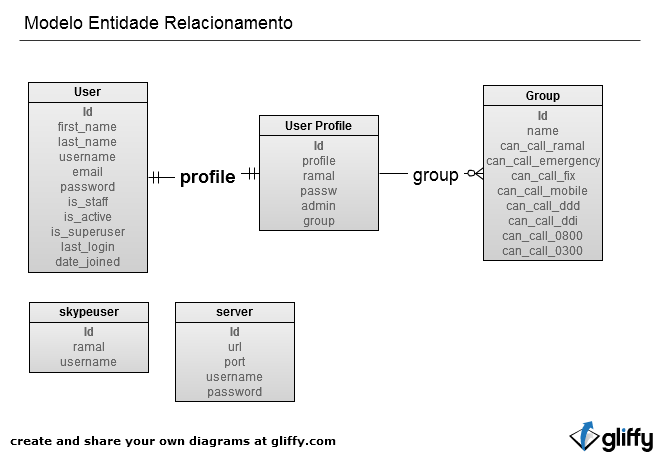
\includegraphics{MER_PABX.png}


\subsubsection{Views}
\label{codigo:views}
Relativo ao arquivo \emph{views.py}. Embora o nome seja confuso esse arquivo é mais parecido com o \emph{Controller} da arquitetura MVC.

É reponsável por:
\begin{itemize}
\item {} 
Toda lógica de negócios (direta ou indireta)

\item {} 
Atribuir variáveis a serem exibidas num \emph{template}

\item {} 
Fazer chamadas ao banco de dados

\end{itemize}


\subsubsection{Decorators}
\label{codigo:decorators}
Relativo ao arquivo \emph{decorators.py}. Aqui são declaradas algumas funções de uso geral que são chamadas diversas vezes nas views. É um arquivo opcional, ou seja, ele existirá somente se o App precisar.


\subsubsection{Templates}
\label{codigo:templates}
Relativo aos arquivos dentro da pasta ``templates''. Embora o nome seja confuso esse arquivo é mais pareciso com a \emph{View} da arquitetura MVC, pois é aqui onde a interface do usuário é renderizada a partir de elementos construídos no arquivo \emph{views.py}

Eventualmente algum App possa precisar de arquivos templates adicionais que estarão contidos na pasta ``templates'' dentro da pasta do App. Além desses arquivos templates, os outros templates padrão estarão contidos na pasta ``templates'' dentro da pasta raiz.


\subsection{Integração com o Asterisk}
\label{codigo:integracao-com-o-asterisk}
Por enquanto a aplicação web do PABX-IP não está integrado com o Asterisk (o software responsável pelo PBX). Para isso seria necessário escrever os dados necessários nos arquivos de configurações utilizados pelo Asterisk, usando sua própria sintaxe.

A integração entre a aplicação web e o Asterisk foi pensada da seguinte forma:
\begin{itemize}
\item {} 
Todas as configurações seriam salvas no banco de dados da aplicação web, evitando assim de ter que ``carregar'' essas configurações a partir do Asterisk toda vez que a aplicação web fosse acessada.

\item {} 
Qualquer alteraçao dessas configurações seria primeiramente salva no banco de dados e em seguida encaminhada para o Asterisk.

\end{itemize}


\section{App Accounts}
\label{apps/accounts:accounts}\label{apps/accounts:app-accounts}\label{apps/accounts::doc}\begin{description}
\item[{Este app é responsável por:}] \leavevmode\begin{itemize}
\item {} 
Definir privilégios de administrador a usuários e limitar acesso a usuários comuns

\item {} 
Cadastro, edição, listagem e remoção de usuários

\item {} 
Autenticação e recuperação de senha

\end{itemize}

\end{description}


\subsection{Modelos}
\label{apps/accounts:module-accounts.models}\label{apps/accounts:modelos}\index{accounts.models (módulo)}
No arquivo models.py estão as classes definidas para armazenar informações extras do usuário. Podemos observar que a classe UserProfile tem uma chave estrangeira na classe User, que é a classe padrão para usuários do Django. Desta maneira, podemos extender os atributos da classe User sem alterar a estrutura de usuário do Django, bastando apenas fazer essa pequena extensão.

Os atributos definidos na classe UserProfile estão detalhados a seguir:
\index{UserProfile (classe em accounts.models)}

\begin{fulllineitems}
\phantomsection\label{apps/accounts:accounts.models.UserProfile}\pysigline{\strong{class }\code{accounts.models.}\bfcode{UserProfile}}~\begin{itemize}
\item {} 
\textbf{profile}: Chave estrangeira que associa um UserProfile a um Usuário. Pode haver apenas um UserProfile por User.

\item {} 
\textbf{ramal}: Ramal associado a um usuário. Esse número é utilizado para fazer ligações.

\item {} 
\textbf{passw}: É a cópia da senha do usuário salva encriptadamente. É utilizada para recuperação de senha.

\item {} 
\textbf{admin}: Indica se o usuário possui o privilégio de administrador.

\item {} 
\textbf{group}: Indica o grupo o qual o usuário pertence.

\end{itemize}

\end{fulllineitems}



\subsection{Formulários}
\label{apps/accounts:module-accounts.forms}\label{apps/accounts:formularios}\index{accounts.forms (módulo)}\index{UserForm (classe em accounts.forms)}

\begin{fulllineitems}
\phantomsection\label{apps/accounts:accounts.forms.UserForm}\pysigline{\strong{class }\code{accounts.forms.}\bfcode{UserForm}}
Formulário utilizado pelo administrador para editar ou criar usuários. Além dos campos padrões relativos a classe User e a classe UserProfile existe um \emph{hidden input} que contém o id do usuário em caso de edição, para que possamos validar as informações na hora de salvar no banco de dados.

O método clean é sobreescrito para validarmos a confirmação de senha e no caso de edição, temos que permitir o salvamento de um ramal ou email já existente.

\end{fulllineitems}

\index{OnlyUserForm (classe em accounts.forms)}

\begin{fulllineitems}
\phantomsection\label{apps/accounts:accounts.forms.OnlyUserForm}\pysigline{\strong{class }\code{accounts.forms.}\bfcode{OnlyUserForm}}
Formulário utilizado para que um usuário sem privilégios de administrador possa mudar seu email ou senha.

\end{fulllineitems}

\index{PassResetForm (classe em accounts.forms)}

\begin{fulllineitems}
\phantomsection\label{apps/accounts:accounts.forms.PassResetForm}\pysigline{\strong{class }\code{accounts.forms.}\bfcode{PassResetForm}}
Formulário utilizado para que um usuário possa receber sua senha esquecida no seu email. Apenas emails cadastrados são aceitos.

\end{fulllineitems}



\subsection{Views}
\label{apps/accounts:module-accounts.views}\label{apps/accounts:views}\index{accounts.views (módulo)}\index{login() (no módulo accounts.views)}

\begin{fulllineitems}
\phantomsection\label{apps/accounts:accounts.views.login}\pysiglinewithargsret{\code{accounts.views.}\bfcode{login}}{\emph{request}}{}
View que inicialmente mostra a tela de login para o usuário, caso o usuário entre na página inicial do projeto ou tente acessar alguma outra página através da url sem estar logado. O usuário ao submeter o formulário de login através de um método POST, fará com que a view tente autenticar esse usuário, e em caso de sucesso, guardará na sessão se o usuário é admininistrador, seu username e seu id e o redirecionará para a página principal. Em caso de falha, a view retorna uma mensagem de erro para o template de login.

\end{fulllineitems}

\index{logout() (no módulo accounts.views)}

\begin{fulllineitems}
\phantomsection\label{apps/accounts:accounts.views.logout}\pysiglinewithargsret{\code{accounts.views.}\bfcode{logout}}{\emph{request}}{}
Faz o logout do usuário logado e o redireciona para a página de login.

\end{fulllineitems}

\index{settings() (no módulo accounts.views)}

\begin{fulllineitems}
\phantomsection\label{apps/accounts:accounts.views.settings}\pysiglinewithargsret{\code{accounts.views.}\bfcode{settings}}{\emph{request}}{}
É a tela que lista todos os usuários do pabx-ip e permite que o administrador escolha qual usuário editar ou remover através de uma interface. Também possui um botão para a tela de cadastro de usuários. É importante lembrar que somente o usuário `root' pode editar ou remover outros administradores.

\end{fulllineitems}

\index{create() (no módulo accounts.views)}

\begin{fulllineitems}
\phantomsection\label{apps/accounts:accounts.views.create}\pysiglinewithargsret{\code{accounts.views.}\bfcode{create}}{\emph{request}}{}
View que usa o UserForm para cadastrar um novo usuário no sistema. Somente acessível para administradores.

\end{fulllineitems}

\index{edit() (no módulo accounts.views)}

\begin{fulllineitems}
\phantomsection\label{apps/accounts:accounts.views.edit}\pysiglinewithargsret{\code{accounts.views.}\bfcode{edit}}{\emph{request}, \emph{offset}}{}
View que usa o UserForm para editar um usuário pré-cadastrado no sistema. Através do offset passado pela url a view sabe o id do usuário que se deseja modificar. Somente acessível para administradores.

\end{fulllineitems}

\index{delete() (no módulo accounts.views)}

\begin{fulllineitems}
\phantomsection\label{apps/accounts:accounts.views.delete}\pysiglinewithargsret{\code{accounts.views.}\bfcode{delete}}{\emph{request}}{}
View usada para remover um usuário do sistema. Através do offset passado pela url a view sabe o id do usuário que se deseja deletar. Primeiramente exibe uma tela de confirmação, e em seguida caso haja confirmação por parte do administrador, a classe User e sua respectiva classe UserProfile são removidas do banco de dados.

\end{fulllineitems}

\index{edit\_self() (no módulo accounts.views)}

\begin{fulllineitems}
\phantomsection\label{apps/accounts:accounts.views.edit_self}\pysiglinewithargsret{\code{accounts.views.}\bfcode{edit\_self}}{\emph{request}}{}
View que o usa o OnlyUserForm para que um usuário comum logado para editar seu email ou senha.

\end{fulllineitems}

\index{save\_or\_update() (no módulo accounts.views)}

\begin{fulllineitems}
\phantomsection\label{apps/accounts:accounts.views.save_or_update}\pysiglinewithargsret{\code{accounts.views.}\bfcode{save\_or\_update}}{\emph{form}, \emph{user=None}, \emph{profile=None}}{}
Método que faz a associação entre um form e os objetos User e UserProfile. Caso os parâmetros user e profile não sejam vazios, a função interpreta como edição de usuário, e terá que fazer a busca dele no banco.

\end{fulllineitems}

\index{password\_reset() (no módulo accounts.views)}

\begin{fulllineitems}
\phantomsection\label{apps/accounts:accounts.views.password_reset}\pysiglinewithargsret{\code{accounts.views.}\bfcode{password\_reset}}{\emph{request}}{}
Retorna inicialmente o template do formulário PassResetForm onde o usuário deverá digitar um email cadastrado válido. Após a submissão do formulário, o sistema checa se existe um servidor smtp pré-cadastrado pelo administrador para envio de emails. Em caso positivo, o email é enviado, e retorna o template indicando uma mensagem de sucesso.

\end{fulllineitems}

\index{encrypt() (no módulo accounts.views)}

\begin{fulllineitems}
\phantomsection\label{apps/accounts:accounts.views.encrypt}\pysiglinewithargsret{\code{accounts.views.}\bfcode{encrypt}}{\emph{plaintext}}{}
Função que retorna a variável \emph{plaintext} encriptada. Usada para salvar a senha encriptada dos usuários no banco.

\end{fulllineitems}

\index{unencrypt() (no módulo accounts.views)}

\begin{fulllineitems}
\phantomsection\label{apps/accounts:accounts.views.unencrypt}\pysiglinewithargsret{\code{accounts.views.}\bfcode{unencrypt}}{\emph{encrypted\_password}}{}
Função que retorna a variável \emph{encrypted\_password} desencriptada. Usada para recuperar a senha dos usuários em caso de esquecimento.

\end{fulllineitems}



\subsection{Templates}
\label{apps/accounts:templates}
Aqui serão listados os templates específicos utilizados por esse App, contidos na pasta ``accounts/templates/''
\begin{itemize}
\item {} 
password\_reset\_form.html: utilizado para renderizar o formulário para recuperação de senha.

\item {} 
password\_reset\_success.html: utilizado para mostrar a mensagem de sucesso na recuperação de senha.

\end{itemize}


\subsection{Decorators}
\label{apps/accounts:module-accounts.decorators}\label{apps/accounts:decorators}\index{accounts.decorators (módulo)}\index{is\_admin() (no módulo accounts.decorators)}

\begin{fulllineitems}
\phantomsection\label{apps/accounts:accounts.decorators.is_admin}\pysiglinewithargsret{\code{accounts.decorators.}\bfcode{is\_admin}}{\emph{function}}{}
Checa se o User logado possui o atributo admin na respectiva classe UserProfile. Usado para limitar o acesso a certas Views que apenas administradores podem acessar.

\end{fulllineitems}



\section{App Groups}
\label{apps/groups:app-groups}\label{apps/groups::doc}\label{apps/groups:groups}\begin{description}
\item[{Este app é responsável por:}] \leavevmode\begin{itemize}
\item {} 
Criar, editar e excluir grupos

\item {} 
Associar permissões de usuários a um ou mais grupos

\end{itemize}

\end{description}

Todas as funcionalidades de grupos é apenas acessível para administradores.

\begin{notice}{warning}{Aviso:}
Esse App não foi finalizado ainda, portanto não atende ainda a todos os requisitos atuais do projeto. Porém no estágio em que ele está desenvolvido é possível rodar o App com as funcionalidades atuais sem problemas.
\end{notice}


\subsection{Modelos}
\label{apps/groups:modelos}\label{apps/groups:module-groups.models}\index{groups.models (módulo)}
Existe uma única classe \emph{Group} definida aqui, que corresponde obviamente a um grupo. Um uso prático para essa classe é poder separar grupos de usuários por departamento, por exemplo: ``grupo recepção'' e ``grupo gerência''.

A associação entre grupos e usuários está definida no model \emph{UserProfile} no qual o atributo \emph{group} define o grupo do usuário. Portanto, um grupo possui vários usuários, mas um usuário só pode se associar a um grupo.

Os atributos da classe grupo são:
\index{Group (classe em groups.models)}

\begin{fulllineitems}
\phantomsection\label{apps/groups:groups.models.Group}\pysigline{\strong{class }\code{groups.models.}\bfcode{Group}}~\begin{itemize}
\item {} 
\textbf{name}: nome do grupo, usado apenas para identificá-lo.

\item {} 
\textbf{can\_call\_ramal}: permissão dada como padrão para todos os grupos, mantemos aqui apenas para fins de visualização.

\item {} 
\textbf{can\_call\_emergency}: permissão dada como padrão para todos os grupos, mantemos aqui apenas para fins de visualização.

\item {} 
\textbf{can\_call\_fix}: indica se o grupo pode fazer ligações para fixo local.

\item {} 
\textbf{can\_call\_mobile}: indica se o grupo pode fazer ligações para celular local.

\item {} 
\textbf{can\_call\_ddd}: indica se grupo pode fazer ligações DDD.

\item {} 
\textbf{can\_call\_ddi}: indica se grupo pode fazer ligações DDI.

\item {} 
\textbf{can\_call\_0800}: indica se grupo pode fazer ligações 0800.

\item {} 
\textbf{can\_call\_0300}: indica se grupo pode fazer ligações 0300.

\end{itemize}

A função \emph{unicode} serve para retornar o nome do grupo no caso de imprimirmos algum objeto Group.

\end{fulllineitems}



\subsection{Formulários}
\label{apps/groups:module-groups.forms}\label{apps/groups:formularios}\index{groups.forms (módulo)}\index{GroupForm (classe em groups.forms)}

\begin{fulllineitems}
\phantomsection\label{apps/groups:groups.forms.GroupForm}\pysigline{\strong{class }\code{groups.forms.}\bfcode{GroupForm}}
\emph{ModelForm} que utiliza como modelo a classe \emph{Group}. A partir dele é possível criar ou editar grupos, e a única instância feita por essa classe é desabilitar o checkbox de permissão para ligar para ramal e para emergência, pois estas permissões são dadas como padrão para qualquer grupo.

\end{fulllineitems}



\subsection{Views}
\label{apps/groups:module-groups.views}\label{apps/groups:views}\index{groups.views (módulo)}\index{index() (no módulo groups.views)}

\begin{fulllineitems}
\phantomsection\label{apps/groups:groups.views.index}\pysiglinewithargsret{\code{groups.views.}\bfcode{index}}{\emph{request}}{}
Função que retorna a lista com os grupos cadastrados, utilizando o template \emph{crud}. Esse template possui links para edição, remoção e criação de grupos.

\end{fulllineitems}

\index{create() (no módulo groups.views)}

\begin{fulllineitems}
\phantomsection\label{apps/groups:groups.views.create}\pysiglinewithargsret{\code{groups.views.}\bfcode{create}}{\emph{request}}{}
View que utiliza o \emph{GroupForm} para criar novos grupos.

\end{fulllineitems}



\section{App Skypelist}
\label{apps/skypelist:app-skypelist}\label{apps/skypelist::doc}\label{apps/skypelist:skypelist}\begin{description}
\item[{Esse app é responsável por:}] \leavevmode\begin{itemize}
\item {} 
Criar, editar e remover contatos skype

\end{itemize}

\end{description}

Um contato Skype é apenas uma associação entre um nome de usuário Skype pré-cadastrado e um ramal do pabx, sendo que este ramal deve ser único, independente de ser um ramal normal ou ``skype''. A idéia por trás disso está em possibilitar o usuário a fazer ligações skype de um telefone normal, conectado ao PABX-IP.

Todas essas funcionalidades desse App está apenas acessível para Administradores.


\subsection{Modelos}
\label{apps/skypelist:module-skypelist.skypeuser}\label{apps/skypelist:modelos}\index{skypelist.skypeuser (módulo)}
Existe uma uńica classe \emph{skypeuser} definida aqui, que corresponde a associação entre nome de usuário skype e ramal.

Os atributos da classe \emph{skypeuser} são:
\index{skypeuser (classe em skypelist.skypeuser)}

\begin{fulllineitems}
\phantomsection\label{apps/skypelist:skypelist.skypeuser.skypeuser}\pysigline{\strong{class }\code{skypelist.skypeuser.}\bfcode{skypeuser}}~\begin{itemize}
\item {} 
\textbf{ramal}: número do ramal.

\item {} 
\textbf{username}: nome de usuário Skype.

\end{itemize}

\end{fulllineitems}



\subsection{Formulários}
\label{apps/skypelist:module-skypelist.forms}\label{apps/skypelist:formularios}\index{skypelist.forms (módulo)}\index{skypeform (classe em skypelist.forms)}

\begin{fulllineitems}
\phantomsection\label{apps/skypelist:skypelist.forms.skypeform}\pysigline{\strong{class }\code{skypelist.forms.}\bfcode{skypeform}}
\emph{ModelForm} que utiliza como modelo a classe \emph{skypeuser}. Acrescenta um campo \emph{hidden input} para tratar o caso de edição do usuário, para evitar a validação de campos com mesmos valores.

\end{fulllineitems}



\subsection{Views}
\label{apps/skypelist:views}\label{apps/skypelist:module-skypelist.views}\index{skypelist.views (módulo)}\index{index() (no módulo skypelist.views)}

\begin{fulllineitems}
\phantomsection\label{apps/skypelist:skypelist.views.index}\pysiglinewithargsret{\code{skypelist.views.}\bfcode{index}}{\emph{request}}{}
Função que retorna a lista com os usuários skype cadastrados, utilizando o template \emph{crud}. Esse template possui links para edição, remoção e criação.

\end{fulllineitems}

\index{create() (no módulo skypelist.views)}

\begin{fulllineitems}
\phantomsection\label{apps/skypelist:skypelist.views.create}\pysiglinewithargsret{\code{skypelist.views.}\bfcode{create}}{\emph{request}}{}
View que utiliza o \emph{skypeform} para criar novos usuários skype.

\end{fulllineitems}

\index{edit() (no módulo skypelist.views)}

\begin{fulllineitems}
\phantomsection\label{apps/skypelist:skypelist.views.edit}\pysiglinewithargsret{\code{skypelist.views.}\bfcode{edit}}{\emph{request}, \emph{offset}}{}
View que utiliza o \emph{skypeform} para editar usuários skype pré-cadastrados. Através do offset passado pela url a view sabe o id do usuário skype que se deseja modificar.

\end{fulllineitems}



\begin{fulllineitems}
\pysigline{\bfcode{delete(request,offset):}}
View usada para remover um usuário skype do sistema. Através do offset passado pela url a view sabe o id do usuário skype que se deseja deletar.Primeiramente exibe uma tela de confirmação, e em seguida caso haja confirmação por parte do administrador, a classe \emph{skypuser} é removida do banco de dados.

\end{fulllineitems}



\section{App Smtp}
\label{apps/smtp:smtp}\label{apps/smtp:app-smtp}\label{apps/smtp::doc}
Esse App é responsável pelo cadastro de um servidor smtp que será usado pelo PABX-IP para enviar emails diversos. A partir de um servidor smtp configurado para o PABX-IP é possível, por exemplo, mandar emails a partir de uma conta cadastrada no gmail.

Apenas um único servidor smtp é permitido, sendo que somente o Administrador pode alterar suas configurações.


\subsection{Modelos}
\label{apps/smtp:module-smtp.server}\label{apps/smtp:modelos}\index{smtp.server (módulo)}
Existe uma única classe \emph{server} definida aqui, que corresponde aos dados do servidor smtp.

Os atributos da classe \emph{server} são:
\index{server (classe em smtp.server)}

\begin{fulllineitems}
\phantomsection\label{apps/smtp:smtp.server.server}\pysigline{\strong{class }\code{smtp.server.}\bfcode{server}}~\begin{itemize}
\item {} 
\textbf{url}: url para o servidor smtp.

\item {} 
\textbf{port}: porta do servidor smtp.

\item {} 
\textbf{username}: nome de usuário do servidor smtp.

\item {} 
\textbf{password}: senha do servidor smtp.

\end{itemize}

\end{fulllineitems}



\subsection{Formulários}
\label{apps/smtp:module-smtp.forms}\label{apps/smtp:formularios}\index{smtp.forms (módulo)}\index{smtpform (classe em smtp.forms)}

\begin{fulllineitems}
\phantomsection\label{apps/smtp:smtp.forms.smtpform}\pysigline{\strong{class }\code{smtp.forms.}\bfcode{smtpform}}
Nesse \emph{ModelForm} cujo modelo é a classe \emph{server}, acrescentamos o campo de confirmação de senha e a validação da mesma. Esse formulário é utilizado tanto para cadastro como edição do servidor smtp.

\end{fulllineitems}



\subsection{Views}
\label{apps/smtp:module-smtp.views}\label{apps/smtp:views}\index{smtp.views (módulo)}\index{index() (no módulo smtp.views)}

\begin{fulllineitems}
\phantomsection\label{apps/smtp:smtp.views.index}\pysiglinewithargsret{\code{smtp.views.}\bfcode{index}}{\emph{request}}{}
Função que retorna os dados do servidor smtp e imprime num template \emph{crud}. Se o servidor não estiver configurado ainda, uma mensagem será exibida. Essa tela ainda possui links para cadastrar ou editar um servidor smtp.

\end{fulllineitems}

\index{configure() (no módulo smtp.views)}

\begin{fulllineitems}
\phantomsection\label{apps/smtp:smtp.views.configure}\pysiglinewithargsret{\code{smtp.views.}\bfcode{configure}}{\emph{request}}{}
Função que permite o cadastro ou a edição do servidor smtp, utilizando o \emph{smtpform}.

\end{fulllineitems}



\section{Templates Padrão}
\label{templates:templates-padrao}\label{templates::doc}
Templates são usados pelo Django para exibir o conteúdo em questão para o usuário, ou seja, é o que o usuário vê de fato.

Os templates padrão são os arquivos html contidos na pasta \emph{templates} logo na raiz do projeto. Apenas alguns arquivos dentre outros contidos nessa mesma pasta são utilizados no projeto, sendo que os não usados são arquivos criados automaticamente pelo Pinax.

Serão listados aqui os templates utilizados:
\begin{itemize}
\item {} 
base.html

\item {} 
crud.html

\item {} 
form\_create.html

\item {} 
form\_delete.html

\item {} 
form\_success.html

\item {} 
login.html

\end{itemize}


\subsection{base.html}
\label{templates:base-html}
É o template base do projeto, que utiliza a mesma estrutura do \emph{fluid layout} do Twitter bootstrap, com alguma modificação para fixar a barra superior. Aqui fica definido o \emph{menu}, o \emph{header} e o \emph{footer}. O conteúdo que eventualmente será carregado na parte do meio, será parte de outro template ``filho'' deste.

A variável ``highlight'' deve ser definida em cada view para manter o link do menu destacado, na seção que o usuário estiver navegando. Assim como a variável ``title'' que define o valor da tag html \emph{title}.


\subsection{crud.html}
\label{templates:crud-html}
Template que extende o template \emph{base.html} e é responsável por criar as tabelas que darão acesso as operações CRUD (acrônimo de Create, Read, Update e Delete em inglês).


\subsection{form\_create.html}
\label{templates:form-create-html}
Template que extende o template \emph{base.html} e é responsável por montar a estrutura dos formulários utilizados por criação e edição de dados.

Aqui também existe um script Javascript que facilita a criação do botão ``cancelar'', pois o link é passado pela \emph{view} correspondente.


\subsection{form\_delete.html}
\label{templates:form-delete-html}
Template que extende o template \emph{base.html} e é responsável por montar a estrutura da tela de confirmação de remoção de algum dado.

Aqui também existe um script Javascript que facilita a criação do botão ``cancelar'', pois o link é passado pela \emph{view} correspondente.


\subsection{form\_success.html}
\label{templates:form-success-html}
Template que extende o template \emph{base.html} e é responsável por montar a estrutura da tela de sucesso no caso de alguma ação (criação,edição ou remoção) ter sido executada com sucesso.

Aqui também existe um script Javascript que facilita a criação do botão ``voltar'', pois o link é passado pela \emph{view} correspondente.


\subsection{login.html}
\label{templates:login-html}
Template que é responsável por montar o formulário de login do usuário.


\section{Bibliotecas externas}
\label{bibliotecas:bibliotecas-externas}\label{bibliotecas::doc}
Nessa seção listaremos as bibliotecas auxiliares ao projeto, que já vem previamente instaladas e configuradas. O desenvolvedor deve ter conhecimento delas caso precise utilizá-las futuramente.

Cada biblioteca utilizada possui também uma documentação própria, que pode elucidar dúvidas mais específicas.


\subsection{Twitter Bootstrap}
\label{bibliotecas:twitter-bootstrap}
\href{http://twitter.github.com/bootstrap/}{http://twitter.github.com/bootstrap/}

Utilizado como base da identidade visual do projeto. Embora o Pinax já venha com um template padrão usando o Twitter Bootstrap, foi preferível começar um novo template para fins de customização.


\subsection{jQuery}
\label{bibliotecas:jquery}
\href{http://jquery.com/}{http://jquery.com/}

É o framework Javascript utilizado no projeto.


\subsection{Sphinx}
\label{bibliotecas:sphinx}
\href{http://sphinx.pocoo.org/}{http://sphinx.pocoo.org/}

Biblioteca utilizada para gerar essa documentação, cujo código fonte se encontra na pasta ``doc'' dentro da pasta raiz do projeto.


\section{Futuras implementações}
\label{futuro::doc}\label{futuro:futuras-implementacoes}
A base do projeto PABX-IP se encontra na manipulação de arquivos, por isso, sugerimos o uso da biblioteca \emph{fileinput} para tal:  \href{http://docs.python.org/library/fileinput.html}{http://docs.python.org/library/fileinput.html}

Conforme visto no StackOverflow:
\href{http://stackoverflow.com/questions/4746190/find-and-replace-within-a-text-file}{http://stackoverflow.com/questions/4746190/find-and-replace-within-a-text-file}


\renewcommand{\indexname}{Índice de Módulos do Python}
\begin{theindex}
\def\bigletter#1{{\Large\sffamily#1}\nopagebreak\vspace{1mm}}
\bigletter{a}
\item {\texttt{accounts.decorators}}, \pageref{apps/accounts:module-accounts.decorators}
\item {\texttt{accounts.forms}}, \pageref{apps/accounts:module-accounts.forms}
\item {\texttt{accounts.models}}, \pageref{apps/accounts:module-accounts.models}
\item {\texttt{accounts.views}}, \pageref{apps/accounts:module-accounts.views}
\indexspace
\bigletter{g}
\item {\texttt{groups.forms}}, \pageref{apps/groups:module-groups.forms}
\item {\texttt{groups.models}}, \pageref{apps/groups:module-groups.models}
\item {\texttt{groups.views}}, \pageref{apps/groups:module-groups.views}
\indexspace
\bigletter{s}
\item {\texttt{skypelist.forms}}, \pageref{apps/skypelist:module-skypelist.forms}
\item {\texttt{skypelist.skypeuser}}, \pageref{apps/skypelist:module-skypelist.skypeuser}
\item {\texttt{skypelist.views}}, \pageref{apps/skypelist:module-skypelist.views}
\item {\texttt{smtp.forms}}, \pageref{apps/smtp:module-smtp.forms}
\item {\texttt{smtp.server}}, \pageref{apps/smtp:module-smtp.server}
\item {\texttt{smtp.views}}, \pageref{apps/smtp:module-smtp.views}
\end{theindex}

\renewcommand{\indexname}{Índice}
\printindex
\end{document}
